% =====================================================================
% Complete Figure Example: Skeleton B — 5-stage horizontal pipeline
% =====================================================================
% USAGE: Complete, COMPILABLE template for agent / sub-agent to copy + customize.
% Strategy: explicit (x, y, w, h) for each zone (NOT fit library)
% guarantees no zone-outside elements.
%
% LAYOUT GRID (5 stages × ~5cm wide, gap 0.5cm):
%   Stage 1: x=[0.0,  4.5],  y=[2,8]   Teal
%   Stage 2: x=[5.0,  9.5],  y=[2,8]   Blue
%   Stage 3: x=[10.0, 14.5], y=[2,8]   Purple (HERO)
%   Stage 4: x=[15.0, 19.5], y=[2,8]   Orange
%   Stage 5: x=[20.0, 24.5], y=[2,8]   Green
%   Bottom Summary Bar: y=[0.5, 1.2]
%   Bottom Color Legend: y=[-0.5, 0]
%
% Each stage uses SAME height = 6cm + same internal padding.
% Each stage = title strip (top 0.5cm) + content area (5.5cm).
%
% Agent / sub-agent customization: change titles + labels + colors. Keep grid.
% =====================================================================

\documentclass[tikz,border=15pt]{standalone}
\usepackage{xcolor,tikz,amsmath,amssymb}
\usetikzlibrary{positioning,calc,backgrounds,arrows.meta,bending}

\definecolor{acaBlueLine}{HTML}{3060A8}
\definecolor{acaBlueBg}{HTML}{DCE6F4}
\definecolor{acaPurpleLine}{HTML}{6E3FA0}
\definecolor{acaPurpleBg}{HTML}{EDE3F6}
\definecolor{acaOrangeLine}{HTML}{D06020}
\definecolor{acaOrangeBg}{HTML}{F9E0D0}
\definecolor{acaGreenLine}{HTML}{389050}
\definecolor{acaGreenBg}{HTML}{DBEDDC}
\definecolor{acaTealLine}{HTML}{1F8F8F}
\definecolor{acaTealBg}{HTML}{D3EBEB}
\definecolor{acaGreyLine}{HTML}{606060}
\definecolor{cellLo}{HTML}{F0E8F8}
\definecolor{cellHi}{HTML}{6E3FA0}

\pgfdeclarelayer{background}
\pgfsetlayers{background,main}

\tikzset{
  base box/.style={
    rectangle, rounded corners=3pt, line width=0.5pt,
    minimum height=0.55cm, font=\scriptsize, align=center, inner sep=3pt,
  },
  flow arrow/.style={
    -{Stealth[length=5pt 1.2, width'=0pt 0.5]},
    line width=1.0pt, shorten >=2pt, shorten <=2pt, color=acaGreyLine,
  },
}

% Helper: draw stage zone with explicit rect + title strip
% Args: #1=line color, #2=bg color, #3=x0, #4=x1, #5=title text
\newcommand{\drawstage}[5]{
  % Zone background
  \begin{pgfonlayer}{background}
    \fill[#2!50, rounded corners=4pt] (#3, 2) rectangle (#4, 8);
  \end{pgfonlayer}
  % Zone border
  \draw[#1, line width=0.7pt, rounded corners=4pt]
    (#3, 2) rectangle (#4, 8);
  % Title strip
  \pgfmathsetmacro\titleX{(#3 + #4) / 2}
  \node[anchor=north, font=\small\bfseries, fill=#1, text=white,
        rounded corners=2pt, inner sep=3pt, inner ysep=2pt,
        minimum width={#4 - #3 - 0.3 cm}]
    at (\titleX, 7.85) {#5};
}

\begin{document}
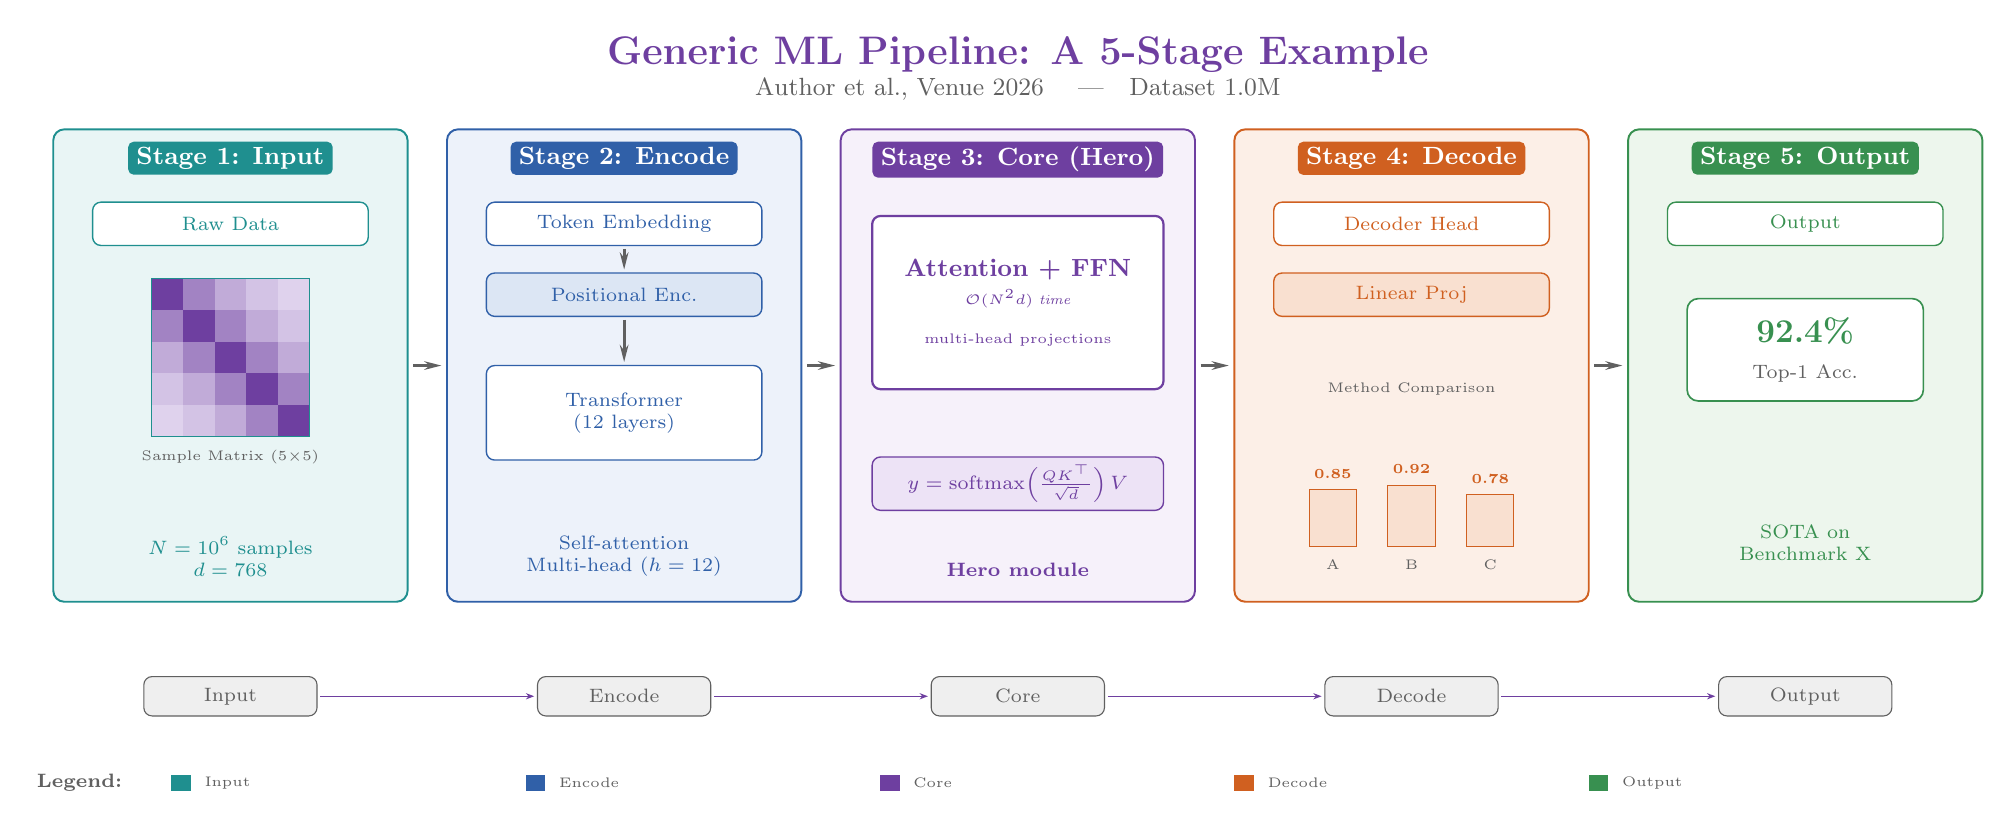
\begin{tikzpicture}

% =====================================================================
% TITLE (top)
% =====================================================================
\node[font=\Large\bfseries, color=acaPurpleLine, anchor=south]
  at (12.25, 8.6) {Generic ML Pipeline: A 5-Stage Example};
\node[font=\small, color=acaGreyLine, anchor=south]
  at (12.25, 8.25) {Author et al., Venue 2026 \quad|\quad Dataset 1.0M};

% =====================================================================
% STAGE 1: INPUT (Teal) — x=[0, 4.5]
% =====================================================================
\drawstage{acaTealLine}{acaTealBg}{0}{4.5}{Stage 1: Input}

% Content (positions confirmed inside [0, 4.5] × [2, 7.4]):
\node[base box, fill=white, draw=acaTealLine, text=acaTealLine,
      minimum width=3.5cm] (s1_data) at (2.25, 6.8) {Raw Data};

% Mini heatmap centered (5×5 at center)
% Fix: Stage 1 zone x=[0, 4.5], center=2.25. Heatmap width=N*cs=2.0
% → xH = 2.25 - 1.0 = 1.25 → heatmap center = 2.25 ✓ (zone center)
\def\xH{1.25}\def\yH{6.1}\def\cs{0.4}\def\N{5}
\foreach \i in {1,...,\N} {
  \foreach \j in {1,...,\N} {
    \pgfmathsetmacro\val{exp(-abs(\i-\j)/2)*100}
    \pgfmathsetmacro\val{int(\val)}
    \pgfmathsetmacro\cx{\xH + (\j - 0.5) * \cs}
    \pgfmathsetmacro\cy{\yH - (\i - 0.5) * \cs}
    \fill[cellHi!\val!cellLo]
      (\cx - \cs/2, \cy - \cs/2) rectangle (\cx + \cs/2, \cy + \cs/2);
  }
}
\draw[acaTealLine, line width=0.4pt]
  (\xH, \yH) rectangle (\xH + \N*\cs, \yH - \N*\cs);
\node[font=\tiny, color=acaGreyLine, anchor=north]
  at (\xH + \N*\cs/2, \yH - \N*\cs - 0.05) {Sample Matrix ($5{\times}5$)};

\node[font=\scriptsize, color=acaTealLine, anchor=south, align=center]
  at (2.25, 2.2) {$N = 10^6$ samples\\$d = 768$};

% =====================================================================
% STAGE 2: ENCODE (Blue) — x=[5, 9.5]
% =====================================================================
\drawstage{acaBlueLine}{acaBlueBg}{5.0}{9.5}{Stage 2: Encode}

\node[base box, fill=white, draw=acaBlueLine, text=acaBlueLine,
      minimum width=3.5cm] (s2_emb) at (7.25, 6.8) {Token Embedding};
\node[base box, fill=acaBlueBg, draw=acaBlueLine, text=acaBlueLine,
      minimum width=3.5cm] (s2_pe) at (7.25, 5.9) {Positional Enc.};
\node[base box, fill=white, draw=acaBlueLine, text=acaBlueLine,
      minimum width=3.5cm, minimum height=1.2cm] (s2_tr)
  at (7.25, 4.4) {Transformer\\(12 layers)};

\draw[flow arrow, shorten >=1pt, shorten <=1pt]
  (s2_emb.south) -- (s2_pe.north);
\draw[flow arrow, shorten >=1pt, shorten <=1pt]
  (s2_pe.south) -- (s2_tr.north);

\node[font=\scriptsize, color=acaBlueLine, anchor=south, align=center]
  at (7.25, 2.2) {Self-attention\\Multi-head ($h=12$)};

% =====================================================================
% STAGE 3: CORE (Purple HERO) — x=[10, 14.5]
% =====================================================================
\drawstage{acaPurpleLine}{acaPurpleBg}{10.0}{14.5}{Stage 3: Core (Hero)}

\node[base box, fill=white, draw=acaPurpleLine, text=acaPurpleLine,
      minimum width=3.7cm, minimum height=2.2cm,
      line width=0.8pt, align=center] (s3_hero)
  at (12.25, 5.8) {%
    {\small\bfseries Attention + FFN}\\[2pt]
    {\tiny\itshape $\mathcal{O}(N^2 d)$ time}\\[6pt]
    {\tiny multi-head projections}};

\node[base box, fill=acaPurpleBg, draw=acaPurpleLine, text=acaPurpleLine,
      minimum width=3.7cm, align=center, font=\scriptsize] (s3_form)
  at (12.25, 3.5)
  {$y = \text{softmax}\!\left(\frac{QK^\top}{\sqrt{d}}\right) V$};

\node[font=\scriptsize, color=acaPurpleLine, anchor=south]
  at (12.25, 2.2) {\textbf{Hero module}};

% =====================================================================
% STAGE 4: DECODE (Orange) — x=[15, 19.5]
% =====================================================================
\drawstage{acaOrangeLine}{acaOrangeBg}{15.0}{19.5}{Stage 4: Decode}

\node[base box, fill=white, draw=acaOrangeLine, text=acaOrangeLine,
      minimum width=3.5cm] (s4_dec) at (17.25, 6.8) {Decoder Head};
\node[base box, fill=acaOrangeBg, draw=acaOrangeLine, text=acaOrangeLine,
      minimum width=3.5cm] (s4_lin) at (17.25, 5.9) {Linear Proj};

% Mini bar chart (3 bars, no foreach to avoid idx issues)
% Title ≥ 0.5cm above value labels (was 0.02cm, severe overlap)
% Fix: Stage 4 zone x=[15, 19.5], center=17.25. 3 bars total width 2.6cm
% → xBC = 17.25 - 1.3 = 15.95 → bars span [15.95, 18.55], center=17.25 ✓
\def\xBC{15.95}\def\yBC{2.7}
\node[font=\tiny, color=acaGreyLine, anchor=south]
  at (\xBC + 1.3, \yBC + 1.8) {Method Comparison};
\foreach \name/\val/\xoff in {A/0.85/0.0, B/0.92/1.0, C/0.78/2.0} {
  \pgfmathsetmacro\bx{\xBC + \xoff}
  \pgfmathsetmacro\bh{0.85 * \val}
  \fill[acaOrangeBg] (\bx, \yBC) rectangle (\bx + 0.6, \yBC + \bh);
  \draw[acaOrangeLine, line width=0.4pt]
    (\bx, \yBC) rectangle (\bx + 0.6, \yBC + \bh);
  \node[font=\tiny\bfseries, color=acaOrangeLine, anchor=south]
    at (\bx + 0.3, \yBC + \bh + 0.02) {\val};
  \node[font=\tiny, color=acaGreyLine, anchor=north]
    at (\bx + 0.3, \yBC - 0.05) {\name};
}

% =====================================================================
% STAGE 5: OUTPUT (Green) — x=[20, 24.5]
% =====================================================================
\drawstage{acaGreenLine}{acaGreenBg}{20.0}{24.5}{Stage 5: Output}

\node[base box, fill=white, draw=acaGreenLine, text=acaGreenLine,
      minimum width=3.5cm] (s5_out) at (22.25, 6.8) {Output};

% Metric card (use \large not \Large — matches surrounding box font)
\node[draw=acaGreenLine, fill=white, rounded corners=4pt,
      line width=0.6pt, minimum width=3.0cm, minimum height=1.3cm,
      align=center, inner sep=4pt] at (22.25, 5.2)
  {{\large\bfseries\color{acaGreenLine} 92.4\%}\\[1pt]
   {\scriptsize\color{acaGreyLine} Top-1 Acc.}};

\node[font=\scriptsize, color=acaGreenLine, anchor=south, align=center]
  at (22.25, 2.4) {SOTA on\\Benchmark X};

% =====================================================================
% INTER-STAGE ARROWS
% =====================================================================
\foreach \a/\b in {4.5/5.0, 9.5/10.0, 14.5/15.0, 19.5/20.0} {
  \draw[flow arrow] (\a, 5) -- (\b, 5);
}

% =====================================================================
% BOTTOM ROW: Summary Bar
% =====================================================================
\foreach \i/\lab in {1/Input, 2/Encode, 3/Core, 4/Decode, 5/Output} {
  \pgfmathsetmacro\sbX{2.25 + (\i - 1) * 5}
  \node[rectangle, rounded corners=3pt, fill=acaGreyLine!10,
        draw=acaGreyLine, line width=0.4pt, font=\scriptsize,
        text=acaGreyLine, inner sep=4pt, minimum height=0.5cm,
        minimum width=2.2cm]
    (sb\i) at (\sbX, 0.8) {\lab};
}
\foreach \a/\b in {1/2, 2/3, 3/4, 4/5} {
  \draw[-{Stealth[length=3pt]}, line width=0.5pt, color=acaPurpleLine,
        shorten >=1pt, shorten <=1pt]
    (sb\a.east) -- (sb\b.west);
}

% =====================================================================
% BOTTOM-MOST: Color Legend
% =====================================================================
\node[font=\scriptsize\bfseries, color=acaGreyLine, anchor=east]
  at (1.0, -0.3) {Legend:};
\foreach \i/\col/\lab in {%
  1/acaTealLine/Input,%
  2/acaBlueLine/Encode,%
  3/acaPurpleLine/Core,%
  4/acaOrangeLine/Decode,%
  5/acaGreenLine/Output%
} {
  \pgfmathsetmacro\lx{1.5 + (\i - 1) * 4.5}
  \fill[\col] (\lx, -0.4) rectangle (\lx + 0.25, -0.2);
  \node[anchor=west, font=\tiny, color=acaGreyLine]
    at (\lx + 0.3, -0.3) {\lab};
}

\end{tikzpicture}
\end{document}
